% Max-Cut -> SDP -> ADMM -> VQLS pipeline.
% Compile:  pdflatex vqls_admm_pipeline.tex
\documentclass[border=12pt]{standalone}
\usepackage{tikz}
\usepackage{amsmath,amssymb}
\usetikzlibrary{arrows.meta,positioning,fit,backgrounds,calc}

\definecolor{clsBlue}{HTML}{1F4E79}
\definecolor{qtmRed}{HTML}{A03030}
\definecolor{ifcGray}{HTML}{4A4A4A}
\definecolor{evalGrn}{HTML}{2D6A4F}
\definecolor{bgClas}{HTML}{EAF1F8}
\definecolor{bgIfc}{HTML}{F2F2F0}
\definecolor{bgQtm}{HTML}{FBEDED}
\definecolor{bgEval}{HTML}{E9F3ED}

\begin{document}
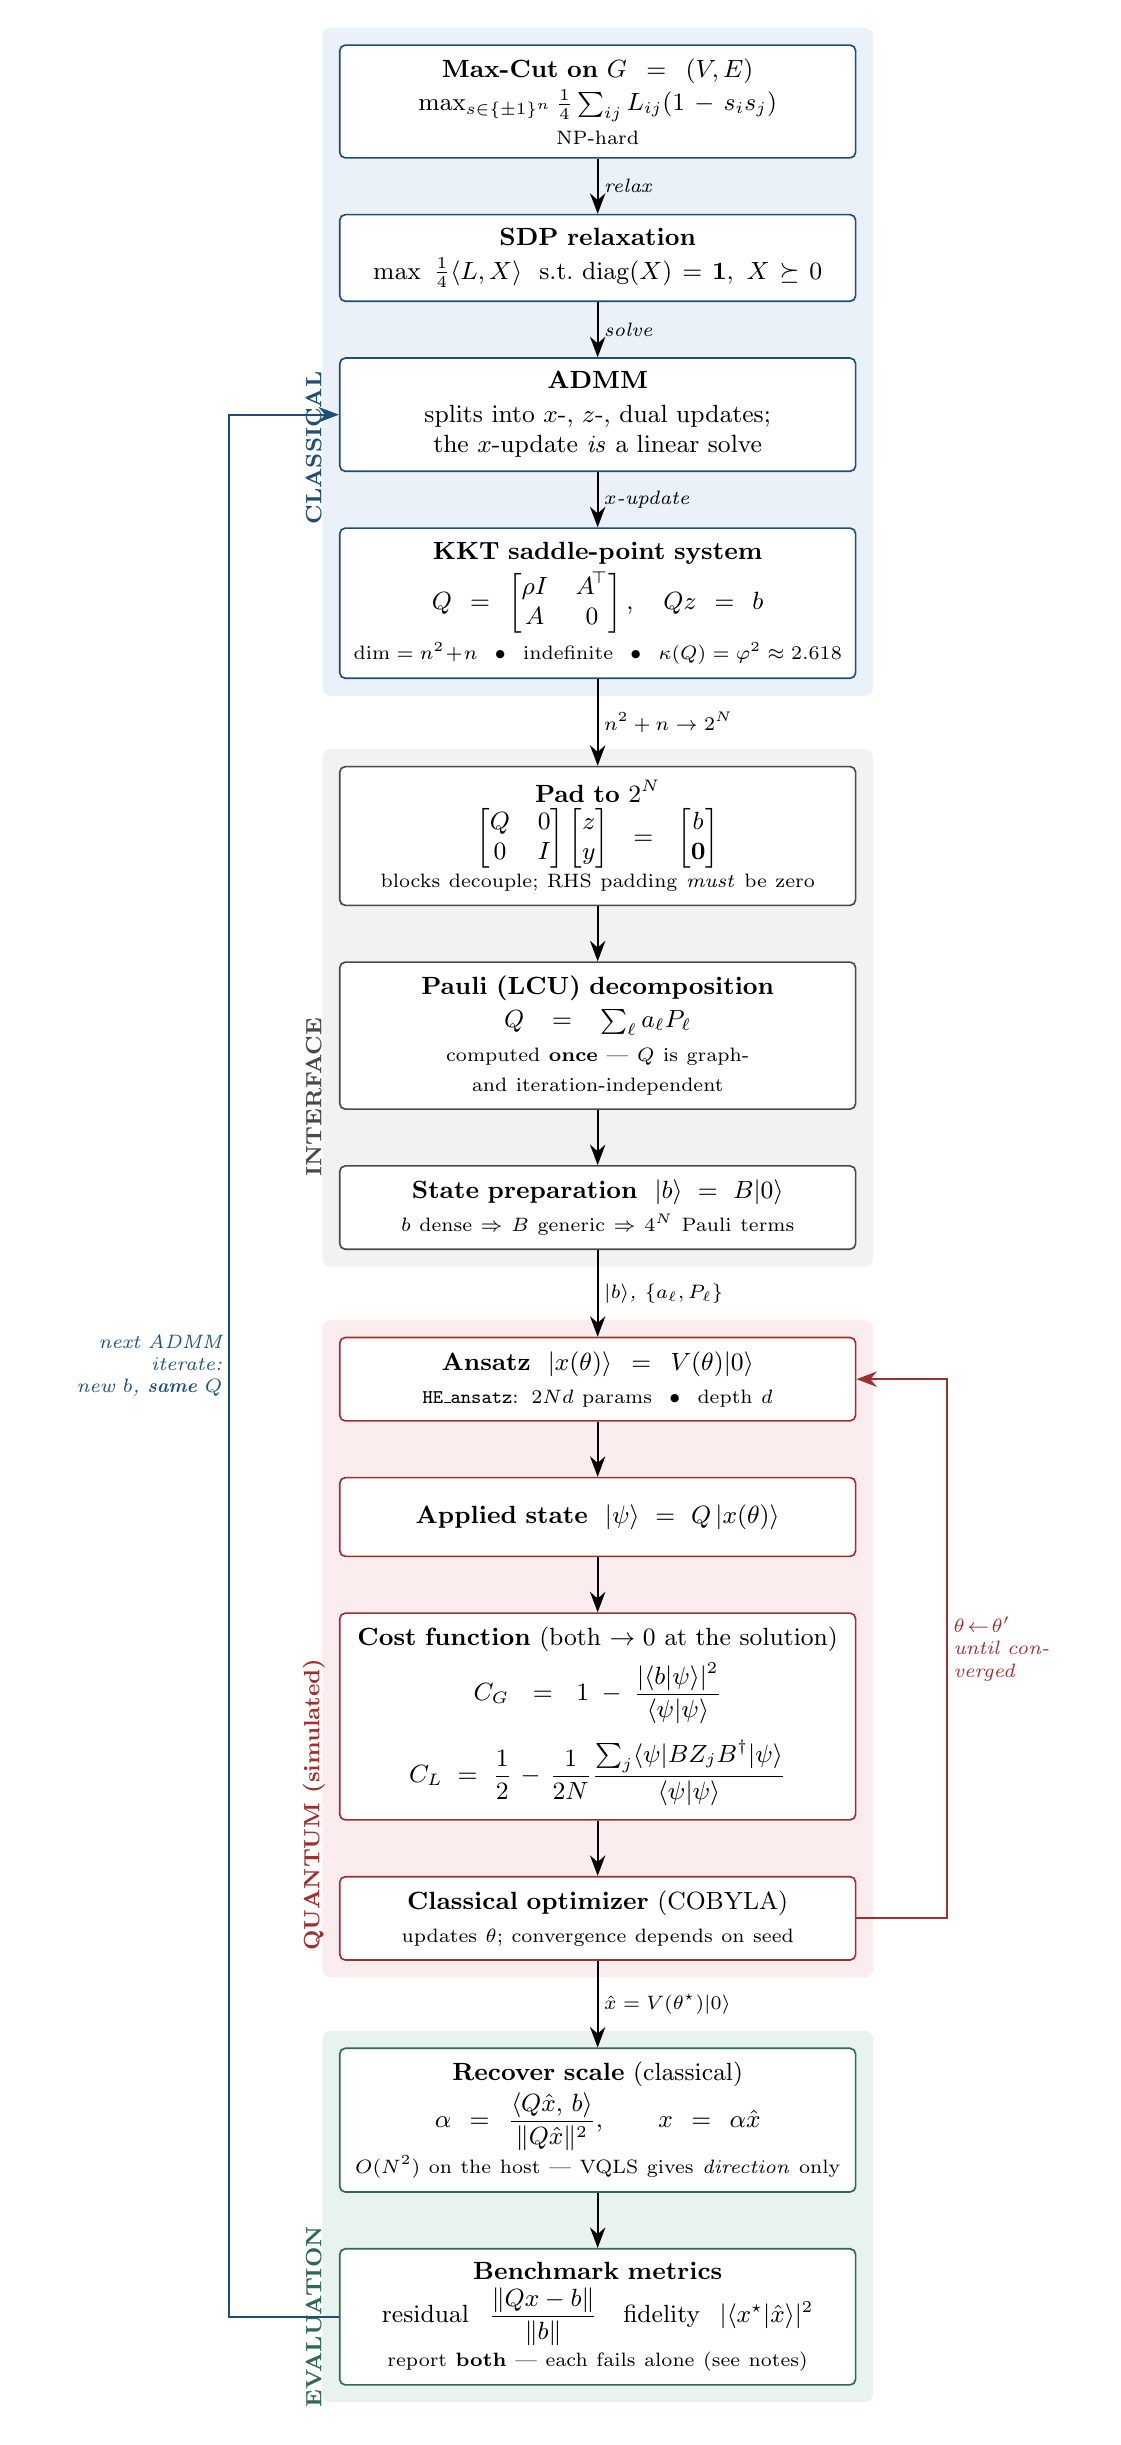
\begin{tikzpicture}[
  font=\small,
  node distance=7mm,
  box/.style={
    draw, rounded corners=2pt, align=center, inner sep=5pt,
    minimum height=10mm, text width=62mm, line width=0.6pt},
  cls/.style={box, draw=clsBlue, fill=white},
  ifc/.style={box, draw=ifcGray, fill=white},
  qtm/.style={box, draw=qtmRed,  fill=white},
  evl/.style={box, draw=evalGrn, fill=white},
  ar/.style={-{Stealth[length=2.6mm]}, line width=0.7pt},
  loopar/.style={-{Stealth[length=2.6mm]}, line width=0.7pt, qtmRed},
  lbl/.style={font=\scriptsize\itshape, inner sep=2pt},
  note/.style={font=\scriptsize, align=left, text width=48mm, inner sep=2pt},
  stage/.style={font=\bfseries\footnotesize, rotate=90, anchor=south},
]

% ---------------- classical layer ----------------
\node[cls] (maxcut) {\textbf{Max-Cut on $G=(V,E)$}\\[1pt]
  $\max_{s\in\{\pm1\}^{n}} \tfrac14\sum_{ij} L_{ij}(1-s_is_j)$\\[1pt]
  \scriptsize NP-hard};

\node[cls, below=of maxcut] (sdp) {\textbf{SDP relaxation}\\[1pt]
  $\max\ \tfrac14\langle L,X\rangle$\ \ s.t.\ $\operatorname{diag}(X)=\mathbf 1,\ X\succeq0$};

\node[cls, below=of sdp] (admm) {\textbf{ADMM}\\[1pt]
  splits into $x$-, $z$-, dual updates;\\
  the $x$-update \emph{is} a linear solve};

\node[cls, below=of admm] (kkt) {\textbf{KKT saddle-point system}\\[2pt]
  $Q=\begin{bmatrix}\rho I & A^{\!\top}\\ A & 0\end{bmatrix},
   \quad Qz=b$\\[2pt]
  \scriptsize $\dim = n^2+n$\ \ $\bullet$\ \ indefinite\ \ $\bullet$\ \ $\kappa(Q)=\varphi^2\approx2.618$};

% ---------------- interface layer ----------------
\node[ifc, below=11mm of kkt] (pad) {\textbf{Pad to $2^{N}$}\\[1pt]
  $\begin{bmatrix}Q&0\\0&I\end{bmatrix}
   \begin{bmatrix}z\\y\end{bmatrix}=
   \begin{bmatrix}b\\ \mathbf 0\end{bmatrix}$\\[1pt]
  \scriptsize blocks decouple; RHS padding \emph{must} be zero};

\node[ifc, below=of pad] (lcu) {\textbf{Pauli (LCU) decomposition}\\[1pt]
  $Q=\sum_{\ell} a_\ell P_\ell$\\[1pt]
  \scriptsize computed \textbf{once} --- $Q$ is graph- and iteration-independent};

\node[ifc, below=of lcu] (prep) {\textbf{State preparation}\ \ $|b\rangle = B|0\rangle$\\[1pt]
  \scriptsize $b$ dense $\Rightarrow$ $B$ generic $\Rightarrow$ $4^{N}$ Pauli terms};

% ---------------- quantum layer ----------------
\node[qtm, below=11mm of prep] (ansatz) {\textbf{Ansatz}\ \ $|x(\theta)\rangle=V(\theta)|0\rangle$\\[1pt]
  \scriptsize \texttt{HE\_ansatz}: $2Nd$ params\ \ $\bullet$\ \ depth $d$};

\node[qtm, below=of ansatz] (apply) {\textbf{Applied state}\ \ $|\psi\rangle = Q\,|x(\theta)\rangle$};

\node[qtm, below=of apply] (cost)
  {\textbf{Cost function} (both $\to 0$ at the solution)\\[3pt]
   $C_G = 1-\dfrac{|\langle b|\psi\rangle|^{2}}{\langle\psi|\psi\rangle}$\\[5pt]
   $C_L = \dfrac12-\dfrac{1}{2N}\dfrac{\sum_j \langle\psi|BZ_jB^{\dagger}|\psi\rangle}
                                       {\langle\psi|\psi\rangle}$};

\node[qtm, below=of cost] (opt) {\textbf{Classical optimizer} (COBYLA)\\[1pt]
  \scriptsize updates $\theta$; convergence depends on seed};

% ---------------- evaluation layer ----------------
\node[evl, below=11mm of opt] (scale) {\textbf{Recover scale} (classical)\\[1pt]
  $\alpha=\dfrac{\langle Q\hat x,\,b\rangle}{\|Q\hat x\|^{2}},\qquad x=\alpha\hat x$\\[1pt]
  \scriptsize $O(N^2)$ on the host --- VQLS gives \emph{direction} only};

\node[evl, below=of scale] (metrics) {\textbf{Benchmark metrics}\\[2pt]
  residual $\;\dfrac{\|Qx-b\|}{\|b\|}$\quad
  fidelity $\;|\langle x^\star|\hat x\rangle|^{2}$\\[1pt]
  \scriptsize report \textbf{both} --- each fails alone (see notes)};

% ---------------- arrows ----------------
\draw[ar] (maxcut) -- node[lbl,right]{relax} (sdp);
\draw[ar] (sdp)    -- node[lbl,right]{solve} (admm);
\draw[ar] (admm)   -- node[lbl,right]{$x$-update} (kkt);
\draw[ar] (kkt)    -- node[lbl,right]{$n^2+n \to 2^{N}$} (pad);
\draw[ar] (pad)    -- (lcu);
\draw[ar] (lcu)    -- (prep);
\draw[ar] (prep)   -- node[lbl,right]{$|b\rangle$, $\{a_\ell,P_\ell\}$} (ansatz);
\draw[ar] (ansatz) -- (apply);
\draw[ar] (apply)  -- (cost);
\draw[ar] (cost)   -- (opt);

% variational feedback loop
\draw[loopar] (opt.east) -- ++(1.15,0)
  |- node[lbl, right, pos=0.25, text width=17mm]{$\theta\!\leftarrow\!\theta'$\\ until converged} (ansatz.east);

\draw[ar] (opt) -- node[lbl,right]{$\hat x = V(\theta^\star)|0\rangle$} (scale);
\draw[ar] (scale) -- (metrics);

% outer ADMM loop: only b changes
\draw[loopar, clsBlue] (metrics.west) -- ++(-1.4,0)
  |- node[lbl, left, pos=0.25, text width=24mm, align=right]
     {next ADMM iterate:\\ new $b$, \textbf{same} $Q$}  (admm.west);

% ---------------- stage backgrounds ----------------
\begin{scope}[on background layer]
  \node[fit=(maxcut)(kkt), fill=bgClas, rounded corners=3pt,
        inner sep=6pt] (bgc) {};
  \node[fit=(pad)(prep),   fill=bgIfc,  rounded corners=3pt,
        inner sep=6pt] (bgi) {};
  \node[fit=(ansatz)(opt), fill=bgQtm,  rounded corners=3pt,
        inner sep=6pt] (bgq) {};
  \node[fit=(scale)(metrics), fill=bgEval, rounded corners=3pt,
        inner sep=6pt] (bge) {};
\end{scope}

\node[stage, clsBlue, left=1mm of bgc.west] {CLASSICAL};
\node[stage, ifcGray, left=1mm of bgi.west] {INTERFACE};
\node[stage, qtmRed,  left=1mm of bgq.west] {QUANTUM (simulated)};
\node[stage, evalGrn, left=1mm of bge.west] {EVALUATION};

\end{tikzpicture}
\end{document}
